 \chapter{Recerca prèvia}
\label{c:recerca prèvia}
\section{La Història de la Intel·ligència Artificial: Des dels Orígens fins Avui}
\subsection{El Naixement d'una Idea Revo lucionaria (1956)}
Tot va començar amb una pregunta provocadora d’Alan Turing, el geni matemàtic que va desxifrar Enigma, una màquina emprada pels nazis per codificar els seus missatges durant la Segona Guerra Mundial (1939-1945): "Podran les màquines pensar alguna vegada?". Aquesta qüestió va obrir les portes a un nou camp d’estudi. En 1956 John McCarthy, Marvin Minsky i d'altres especialistes van nominar oficialment el terme ``intel·ligència artificial'' durant la famosa conferència de Dartmouth, marcant l'inici d'una nova era tecnològica.
\subsection{El Joc que ho va canviar tot: The Imitation Game/El test de Turing}
El nucli de la IA es basa en un experiment molt senzill, però profund: El joc d'imitació (The imitation game), proposat per Alan Turing. Davant de la pregunta "Podran les màquines pensar alguna vegada?", Turing va dissenyar un joc que funcionava com a test per les màquines anomenat ``The Imitation Game''. Aquest test consistia en el fet que un avaluador havia de començar una conversa en forma de textos escrits amb una persona i una màquina durant 5 minuts, aquest avaluador no sabia qui era qui i el seu objectiu era esbrinar qui era l'humà. Si la màquina aconseguia enganyar a l'avaluador passava el test i es reconeixia que la màquina havia aconseguit un nivell de comportament lingüístic equivalent a la d'un humà, i donava resposta a la pregunta d'Alan Turing. Al cap dels anys, el joc ha estat evolucionant i moderat pels prodigis de la humanitat fins que avui en dia és conegut com el test de Turing. Tot això va ser clau en donar lloc al naixement de la IA i per l'avanç de la tecnologia.
\subsection{ELs grans fites de la IA}
\subsubsection{1997: La maquina que va vencer un campio}
 La supercomputadora Deep Blue desnvolupada per IBM va derrotar el campió mundial d’escacs, Garry Kasparov, demostrant que la IA podia superar els humans en jocs d’estratègia complexos.
\subsubsection{2022: L'explosió de la IA}
Milions d’usuaris van descobrir models com ChatGPT que podien escriure, traduir i programar amb un llenguatge gairebé humà, obrint nous horitzons en la interacció home-màquina.
\subsubsection{2025: La IA en tots els ambits}
    2025: La IA en Tots els Àmbits
    Avui, la IA està present en dibuix, contingut audiovisual, cotxes autònoms, medicina i molt més, amb models cada vegada més especialitzats i avançats.



(Fonts: \cite{McCarthy_Minsky_Rochester_Shannon_2006}, \cite{deep-blue},
\href{https://openai.com/index/chatgpt/}{ChatGPT (2022)},
\cite{10.1093/mind/LIX.236.433}
)
\section{Historia de les xarxes neuronals artificials}
La història de les xarxes neuronals és molt extensa, per tant, resumirem molt aquest apartat, parlant molt breument de les creacions de xarxes més importants.
\subsection{Perceptron (1958)}
En la dècada de 1950 a 1960 el psicòleg i informàtic Frank Rosenblatt va crear el Percecptrò, la primera xarxa neuronal creada, a partir d'aquest moment, es potenciarien les xarxes neuronals.

Aquest model pren varies entrades binaries $x_1$, $x_2$, fins les que calguin, i produeix una sola sortida binaria. Per calcular la sortida, Rosenblatt va introduir els ``pesos'', que está explict a l'apartat \ref{sec:3.8}, els seus principals usos són decsions binàries senziles, o per crear funcions lògiques com OR o AND.

\subsection{Multiplayer Perceptron}
El multiplayer perceptron és una ampliació de la percepció d'una única neurona a més d'una. A més, apareix el concepte de capes d'entrades, capes ocultes i capes de sortida, (tot això explicat a l'apartat \ref{sec:3.6}) però amb valors d'entrada i rtida binàries. No hem d'ignorar que els científics asignaban el valor del pes i del umbral manualment en cada neurona, quan més perceptrons havien en les capes, era molt més difícil establir els pesos desitjats.

\subsection{Neurones sigmoide}
Per aconseguir que les xarxes neuronals aprenguin per elles mateixes, es a dir, aprenentatge automàtic \ref{3.4.2}, va ser necessari introduir un nou tipus de neurones, que són les Neurones Sigmoides, que són similar al perceptró, aquestes neurones en comptes de que les entrades siguin 1 o 0, puguin tenir valors com 0.5, o 0.374 o qualsevol altre valor real. Ara les sorides en lloc de ser 0 o 1, serà d(w . x + b), on d serà la funció sigmoide, explicat en l'apartat \ref{3.7.1}. Aquesta va ser la primera funció d'activació \ref{3.5.3}.

\subsection{Xarxa neuronal prealmentada (Feedforward)}
Les xarxes neuronals prealimentades són les que les sortides d'una sola capa són utilitzades com entrades en la pròxima, com explicarem més endevant en l'apartat \ref{sec:3.6} capa, on les conexions entre les unitats no dornen un cicle.

\section{Que és la Ia?}
Hem estat parlant molt durant aquest treball sobre la IA, i ara que em après quina és la seva història, hem de saber que és. Doncs bé, podem definir la IA com sistemes de software i de hardware disenyats per humans que actúen en un la dimensió física o digital, es a dir, raonar sobre el coneixemen, processant la informació derivada de dades i prendre les millors decisions per assolir l'objectiu donat. O dit d'un altre manera, és un camp de la informàtica que consisteix en un conjunt de capacitats interectuals i cognitives expresades per un sistema informàtic creat pels humans que té com a proposit imitar la intel·ligència humana, com escriure poemes, reconeixer imatges, fer prediccions basades en dades i més funcions. Un exemple de IA i que tot el món coneix i utilitza és el ChatGPT, un chatbot impulsada per un model d'intel·ligència artificial generativa de la empresa OpenAI. Utilitza técniques de processament de llenguatge natural per comprendre preguntes fetes per l'usuari i generar respostes coherents en converses, simulant una interacció similar a la d'un humà. Aquesta IA ha avançat molt desde el seu llençament, ara pot generar o editar imatges, procesar audios, llegir arxius, comrendre imatges i molt més.

\section{Com funciona la IA?}
Una vegada que ja sabem que és una IA, ens toca entendre com funciona. Les intel·ligències arficials utilitzen algoritmes i models matemàtics per processar grans quantitats de dades i prendre accions basades en patrons i regles establertes a travès de l'aprenentatge automàtic o l'aprenentatge profund. Per tant per funcionar necessitara:  \nameref{subsec:Dades}  \ \nameref{subsec:Algorismes}  \ \nameref{subsec:Potència computacional} \ \nameref{subsec:Software i Frameworks} \ \nameref{subsec:Optimització i Ajustos}  \ \nameref{subsec:Ètica i Regulació}

\subsection{Dades}\label{subsec:Dades}
Les dades son fonamentals per la IA ja que es la base de l'aprennetatge del model, per poder raonar, prendre decisions, i millorar la presició. Aquí esdevenen uns exemples que pot haver:

\subsubsection{Basé d'aprenentage}
\begin{itemize}
 \item Les algoritmes de la IA necessiten a base de dades i una gran diversitat de dades per poder identificar patrons i construir prediccion.
\end{itemize}
\subsubsection{Qualitat vs Quantitat}
\begin{itemize}
\item Una gran quantitat de dades ajudaran a la IA a obtendendre major precisió, però la qualitat es encara més important per la complexibilitat de dades que aporta, això evitara que la IA cometes errors per informacio incompleta.\textbf{ Per exemple:} {\color{blue}En l'ambit medic si vols que la IA fagi una predicció i tan sol li dones una quantitat important de persones sanes i no d'altres exemplars, la IA simplement descartara d'altres possibilitats que podrian haver i només agafar la sana.}
\end{itemize}
\subsubsection{Exemples Reals}
\begin{itemize}
 \item Les sistemes dels cotxes o assistents virtuals necessiten dades en temps reals per adaptar-se de l'entorn, també plataformes com Netflix o Spotify necessiten dades personalitzades per poder generar recomanacions amb presició.
\end{itemize}
\subsubsection{Legisme i Etica}
\begin{itemize}
 \item A la IA s'ha d'aplicar dades com protecció de dades per favorir l'etica i moral, i se li ha d'entrenar amb fonts legitima, valides per tal d'evitar erros legals o tecnics
\end{itemize}


\subsection{Algorismes}\label{subsec:Algorismes}
\subsubsection{Algoritme Gredient descendent:}\label{subsec:gradient}
L'algoritme de Gradient descendent és un algoritme imprescindible en l'entrenament de les xarxes neuronals, i de la intel·ligència artificial. Primer de tot hem d'entendre que és un gradient i una funció d'error.

\textbf{Gradient:}En les xarxes neuronals, un gradient és un vector que indica la direcció en la que es mou i amb quina intensitat per que la funció d'error cambii més ràpid respecte als pesos de la xarxa neuronal. Per calcular el gradient, s'utilitza la derivada parcial de la funció de pèrdua respecte als pesos.

\textbf{Funció d'error:} La funció d'error tracta de determinar el error entre el valor estimat i el valor real, amb la finalitat d'optimitzar els paràmetres de la xarxa neuronal, aixó està explicat en l'apartat \ref{subsec:pèrdua}.

L' objectiu de l'algoritme gradiant descendent és minimitzar la funció d'error, o també l'error entre la predicció, es a dir, trobar la funció de pèrdua mínima, per aconseguir-ho s'ha de trobar el valor mínim de la funció. La funció de pèrdua mínima significa que els errors dels paràmetres (pesos i biaixos) de la xarxa han de ser molt aproximades al valor real, on s'ajusten aquest paràmetres ja que no són exactes.

\begin{figure}[H]
    \centering
    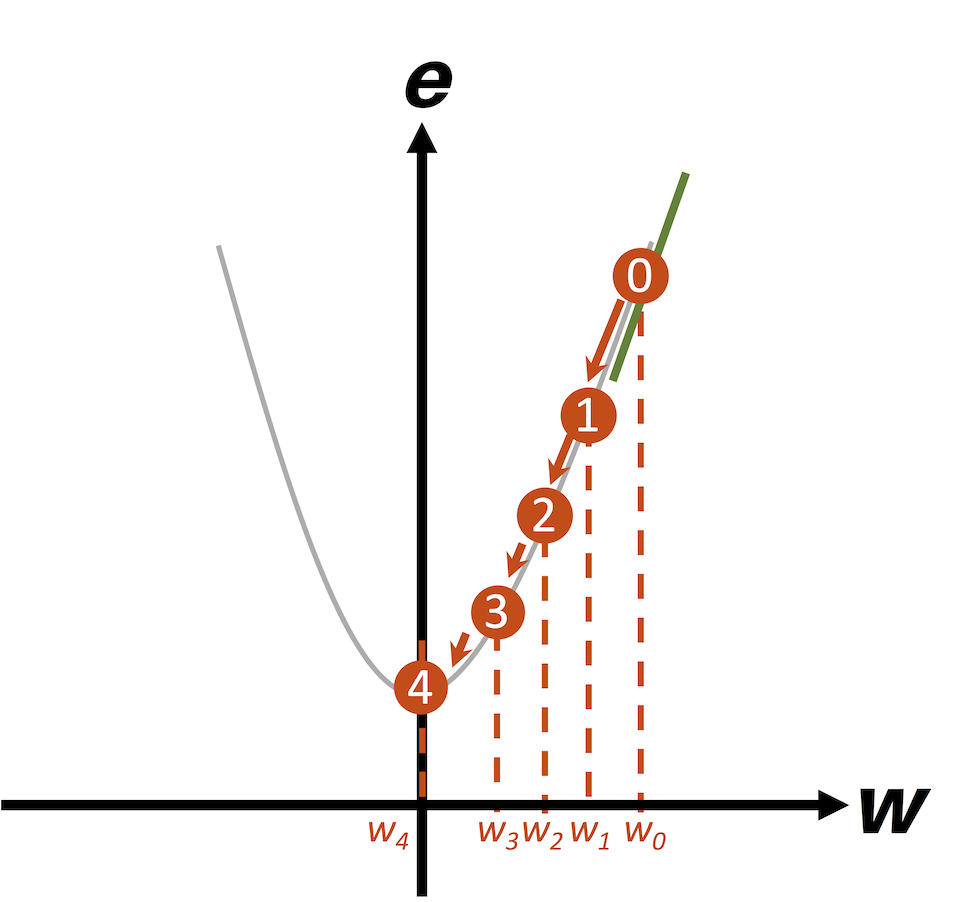
\includegraphics[width=0.5\textwidth]{./figures/gradient_descendent.png}
    \caption{Gràfica de gradient descendent}
\end{figure}

En la figura d'adalt, on podem apreciar quatre iteracions, el valor inicial és un punt qualsevol de la funció. Al inici de la funció, en el punt 0, els paràmetres de la funció s'asignen aleatoriament, i la pèrdua és alta, es a dir, que els errors són grans. Desde aquell punt, trobarem la derivada parcial en cada una de les iteracions, i el gradiet serà l'encarregat de guiar els canvis als paràmetres.
Al principi de tot, el gradient serà molt pronunciat, però a mesura que es van generant nous paràmetres durant l'entrenament, s'anirà reduint fins al put més baix d'aquesta corba, on els errors són molt petits, aquest punt se li diu punt de convergència. Aquí és on la xarxa ha après i ha ajustat millor les dades.

La fòrmula del gradient ascendent és la seguent: \\

$\Delta w_{ij} = a \left( \frac{\partial E}{\partial w_{ij}} \right)$ \\

Aquesta és la formula més ràpida per arribar al punt màxim dels gradients. Per tant la fòrmula del gradient descendent seria aquesta mateixa en negatiu, perquè és la forma més ràpida de trobar el punt mínim.

$\Delta w_{ij} = -a \left( \frac{\partial E}{\partial w_{ij}} \right)$

\textbf{Explicació de la fòrmula:}\\
$\Delta w_{ij}$: Representa quant s'ajusta el pes en una iteració de l'entrenamen.

$a$: És la constant d'aprenentatge, aquesta constant defineix quant afecta el gradiant en l'actualització dels nostres paràmetres en cada iteració. Si aquest valor és gran, cada iteració és molt gran, i el punt serà incapaç d'introduir-se al punt de convergència, causant que el procès d'optimització acabi en un bucle infinit. Tanmateix, si és petit, el punt s'aproxima poc a poc al punt de converència, però calcularà moltes iterai això pot ser ineficient. Per tant aquest valor ha de estar en un punt mig, en que no sigui molt gran ni molt petit.

\begin{figure}[H]
    \centering
    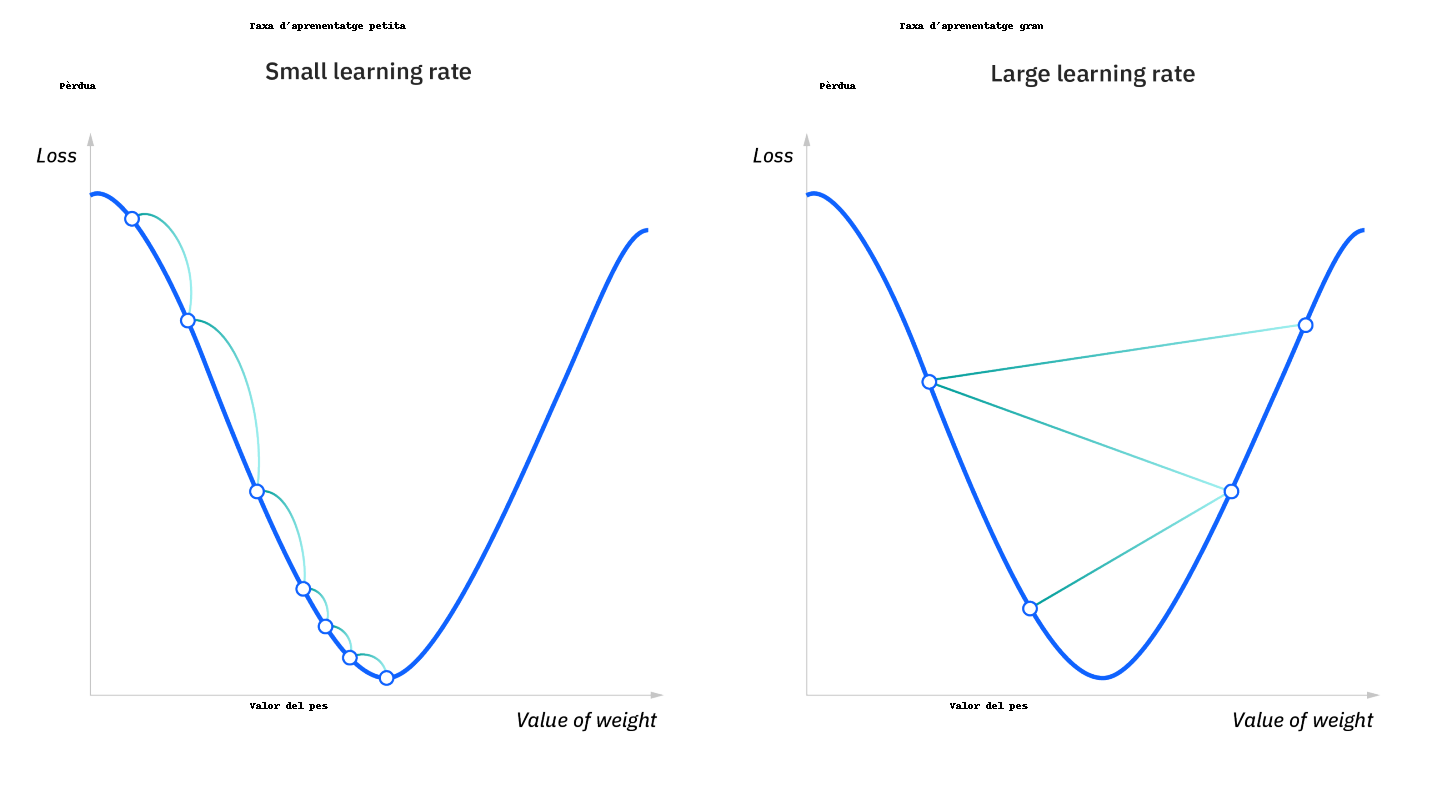
\includegraphics[width=0.5\textwidth]{./figures/constant_gradient.png}
    \caption{Gràfiques de valors gran i petit de la constant d'aprenentatge}
\end{figure}


$\left( \frac{\partial E}{\partial w_{ij}} \right)$: És la derivada parcial de $E$ respecte a $\Delta w_{ij}$. \\

A la figura 3.2, és una representació en 2 d, però en situacions reals el gradient descendent es representa en la dimensió 3 d.


\begin{figure}[H]
    \centering
    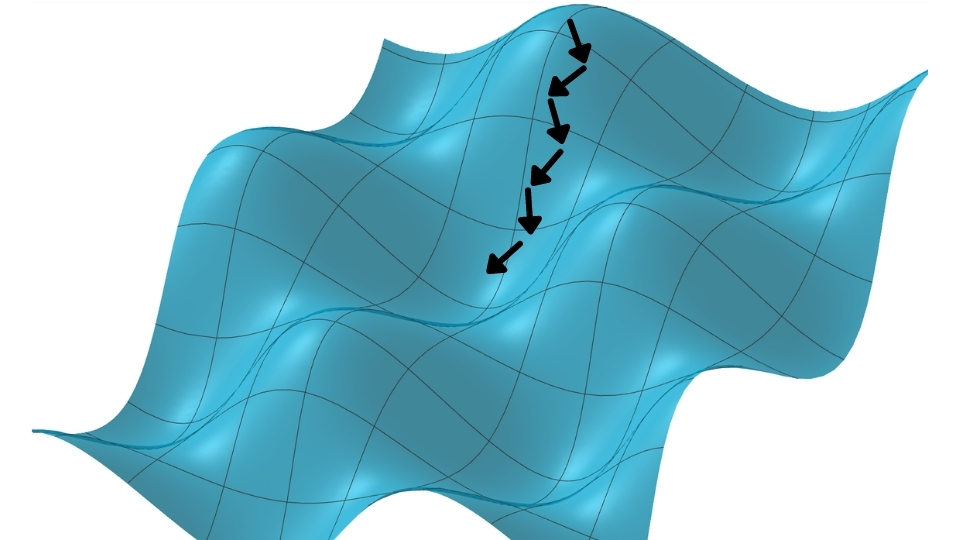
\includegraphics[width=0.5\textwidth]{./figures/gradient_descendent3d.png}
    \caption{Repressentació del gradient descendent en 3d}
\end{figure}

Fonts: \href{https://www.ibm.com/es-es/think/topics/gradient-descent}{ibm.com} i \href{https://www.youtube.com/watch?v=A6FiCDoz8_4&ab_channel=DotCSV}{YouTube}.

\subsubsection{L'aprenentage automàtic(Machine learning)}
\begin{itemize}
 \item L'aprenentatge automàtic és una branca crucial de la intel·ligencia artificial, consisteix en cobrar vida a la maquina, donar-li el poder d'apendre com els humans, realitzar tasques de manera autonoma i finalment, les infinites possibilitats d'evolucionar a traves de l'experiencia i molt més. Segons la \href{https://ischoolonline.berkeley.edu/blog/what-is-machine-learning/}{UC Berkeley} el procés de l'aprenentatge automatic es pot dividir en tres parts:

  \begin{enumerate}
  {\color{gray}
   \item \textbf{Mecanisme de predicció}
    \subitem\hspace*{-1\leftmargin} Un conjunt de regles o operacions matemàtics que analitza les dades d'entrada i intenta identificar els patrons que busca el model.
   \item \textbf{Funció de pèrdua (o error)}\label{subsec:pèrdua}
   \subitem\hspace*{-1\leftmargin} Un sistema per avaluar l'encert de les prediccions, comparant-les amb resultats reals (quan es disposa d'ells). Si la predicció és incorrecta, aquesta funció quantifica la magnitud de l'error.
   \item \textbf{Algorisme d'optimització}
   \subitem\hspace*{-1\leftmargin} El procés que ajusta automàticament el model per minimitzar l'error, modificant els paràmetres interns per millorar les prediccions futures.} \ \footnote{Llengua original: Anglessa; Traduit per el chat bot Deepseek}
  \end{enumerate}
   \end{itemize}
  Segons \href{https://blogs.nvidia.com/blog/supervised-unsupervised-learning/}{Nvidia} hi han molts tipus d'apranentage automatics:
  \begin{description}
   \item \nameref{subsubsec:Aprenentatge supervisat}
   \item \nameref{subsubsec:Aprenentatge semi-supervisat}
   \item \nameref{subsubsec:Aprenentatge no supervisat}
   \item \nameref{subsubsec:Aprenentatge reforç}
  \end{description}
\subsubsection{Aprenentatge supervisat}\label{subsubsec:Aprenentatge supervisat}
L'aprenentatge supervisat és un tipus d'aprenentatge automàtic que treballa amb dades etiquetades, és a dir, dades que ja inclouen la solució o resultat desitjat. En aquest mètode, la intel·ligència artificial aprén a associar les dades d'entrada amb les seves etiquetes corresponents, mitjançant l'anàlisi d'exemples prèviament resolts. Això li permet desenvolupar la capacitat de resoldre problemes nous aplicant la lògica i els patrons identificats a partir de dades reals. \\

\textbf{Avantatges i desavanantatge:}
Aquest mètode destaca per la seva alta precisió en problemes ben definits, ja que al treballar amb dades prèviament etiquetades pot assolir bons resultats en tasques de classificació i regressió. Una altra avantatge important és la facilitat per avaluar el rendiment dels models. A més, es tracta d'una àmplia àrea d'estudi amb una gran varietat d'algoritmes ben desenvolupats i optimitzats, com ara els arbres de decisió, els random forests, les màquines de vectors de suport (SVM) o les xarxes neuronals. Finalment, un cop entrenat adequadament, el model pot generalitzar el seu aprenentatge i fer prediccions útils sobre dades noves.\\

No obstant això, aquest enfocament també presenta alguns inconvenients significatius. El principal desavantatge és la seva forta dependència de conjunts de dades etiquetades, que sovint són costosos d'obtenir i preparar com las de medicines. Un altre problema freqüent és el sobreajustament (overfitting), que ocorre quan el model memoritza les dades d'entrenament en lloc d'aprendre patrons generals, la qual cosa provoca una perdua de raonament logica. Finalment, aquest mètode pot tenir dificultats per manejar certs tipus de dades no estructurades o problemes complexos, que podrien requerir quantitats molt grans de dades etiquetades per assolir un bon rendiment.


\subsubsection{Aprenentatge semi-supervisat}\label{subsubsec:Aprenentatge semi-supervisat}

L'aprenentatge semi-supervisat representa un punt intermig entre l'aprenentatge supervisat i el no supervisat, aprofitant tant dades etiquetades com no etiquetades per millorar l'eficiència dels models d'aprenentatge automàtic. Això funciona quan l'obtencio de les dades etiquetades son molt costoses i l'extraccio de les característiques son molt complexes.
\subsubsection{Aprenentatge no supervisat}\label{subsubsec:Aprenentatge no supervisat}

L'aprenentatge no supervisat és una branca de l'aprenentatge automàtic que s'utilitza quan no es disposa de dades etiquetades. A diferència de l'aprenentatge supervisat, on el model rep exemples amb les seves solucions correctes, en aquest cas l'algorisme ha de descobrir per si mateix l'estructura i els patrons, fent una diagnosticació agrupant les característiques similars que poden haber entre les dades.

Depenen dels tipus de  problemes, les dades s'organitzen de diferents maneres.
\begin{itemize}
 \item \textbf{Clustering:} Tècnica que agrupa les dades en funció de les seves similituds.
 \item \textbf{Anomaly detection:} Cerca patrons que no encaixen amb el comportament normal.
 \item \textbf{Association:} Cerca relacions i correlacions entre variables en grans conjunts de dades.
 \item \textbf{Autoencoders:} Els autoencoders són un tipus de xarxa neuronal artificial que aprèn a comprimir i reconstruir dades.
\end{itemize}


\subsubsection{Aprenentatge per reforç}\label{subsubsec:Aprenentatge reforç}
L'aprenentatge per reforç és una branca de l'aprenentatge automàtic inspirada en la manera com els éssers vius aprenen mitjançant la interacció amb el seu entorn. Com per exemple quan començem a jugar un videojoc, en els jocs rebem senyals de reforços, de si completem un nivell ens ortoga un trofeu, de si matem certs enemics guanyem bonificacions. Amb aquest sistema de penalitzacio i recompenses guia al jugador a millorar les seves tecniques de videojocs, i això  el podem aplicar perfectament en la IA.
Totes les aprenantatges de reforç segueixen pragmaticament aquest esquema per l'aprenentage:
\begin{enumerate}
 \item \textbf{Acció}
 \item \textbf{Observació}
 \item \textbf{Recompensa}
 \item \textbf{Ajust d'estrategia}
\end{enumerate}


\subsubsection{Aprenentatge profund}
\begin{itemize}
    \item L'aprenentatge profund és una branca de l'aprenentatge automàtic que utilitza \nameref{sec:xarxa neuronal} amb múltiples capes per processar dades complexes i extreure'n característiques rellevants. Inspirat en el funcionament del cervell humà, aquest enfocament permet identificar patrons i analitzar dades de alta complexitat. Durant la fase d'identificació, empra un aprenentatge jeràrquic, és a dir, progressa gradualment des de característiques simples fins a patrons complexes.
\end{itemize}



\begin{figure}[h!]
    \centering
    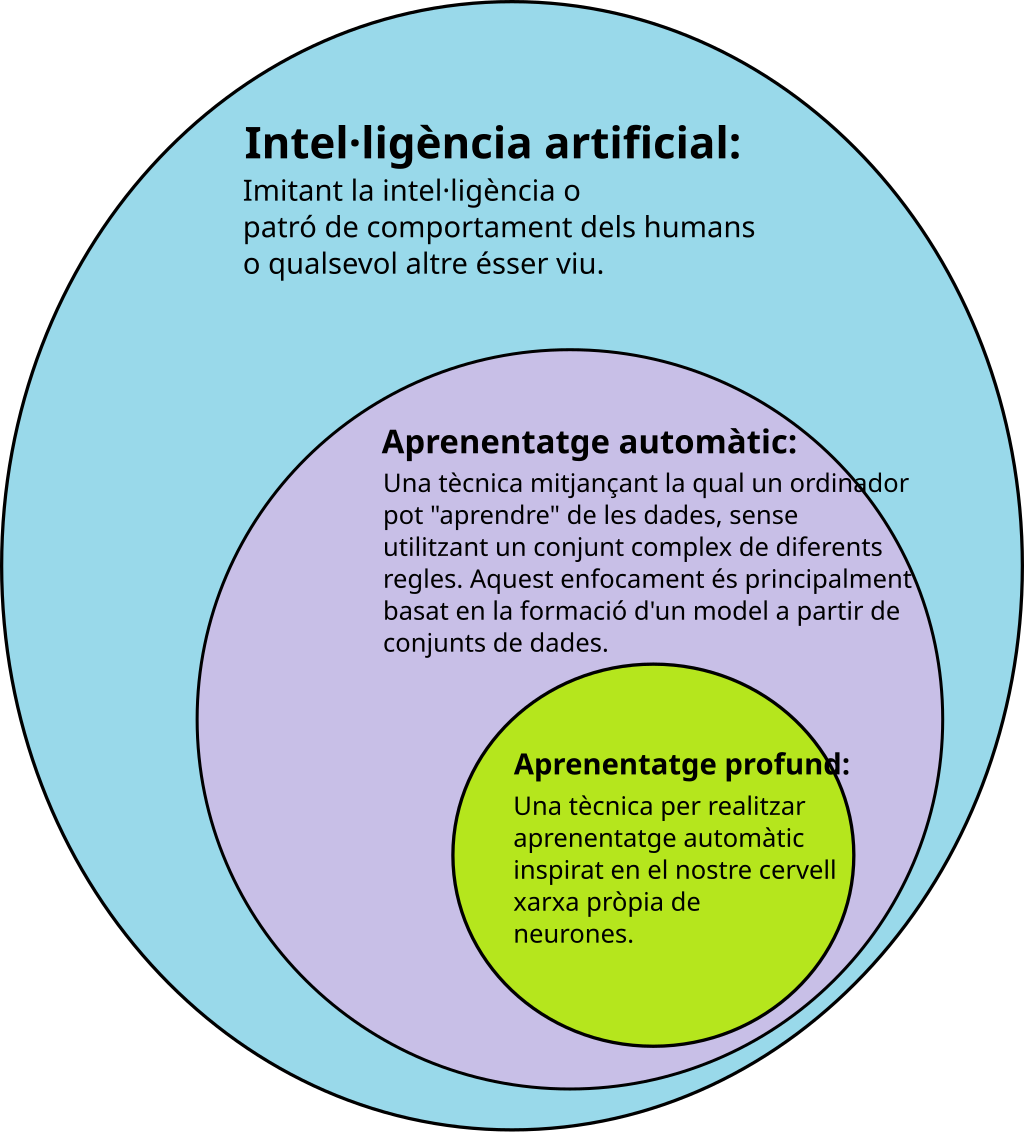
\includegraphics[width=0.2\textwidth]{./figures/Aprenentatge.png}
    \caption{Les capes que te la IA per funcionar}
\end{figure}


\subsection{Potència computacional}\label{subsec:Potència computacional}
La intel·ligència artificial (IA) i la potència de càlcul estan profundament connectades. Sense maquinari potent, les aplicacions d’IA no podrien processar algoritmes complexos ni gestionar les enormes quantitats de dades que requereixen els models actuals. \\

Ultimament em vist el gran avanç que esta fent la IA, per tant la potencia computacional també creix consecutivament. D'aquesta manera la IA cada vegada es pareguera més a un huma i podrà ser més original alhora de crear contingut.\\

Una \hyperref[GPUs]{\textbf{GPUs}} té un papel molt important en la IA de tal manera que pot lograr a accelelar els calculs que fa. Per la cual cosa fa que el seu mercat puguess arribar fins a 53 milions de dolars en 2023 i s'estima a que arribara fins al 473 milions en 2033.\\

Tot això provoca un gran comerç i invertiment en la creació d'un chip exclusiu solament per la IA, donant llavor una rapideza encara més fascinant alhora de fer calculs.\\

Uns dels principals  protagonistes que treballen en el hardware de la IA, son mostrat per la següent imatge:
\begin{figure}[h!]
    \centering
    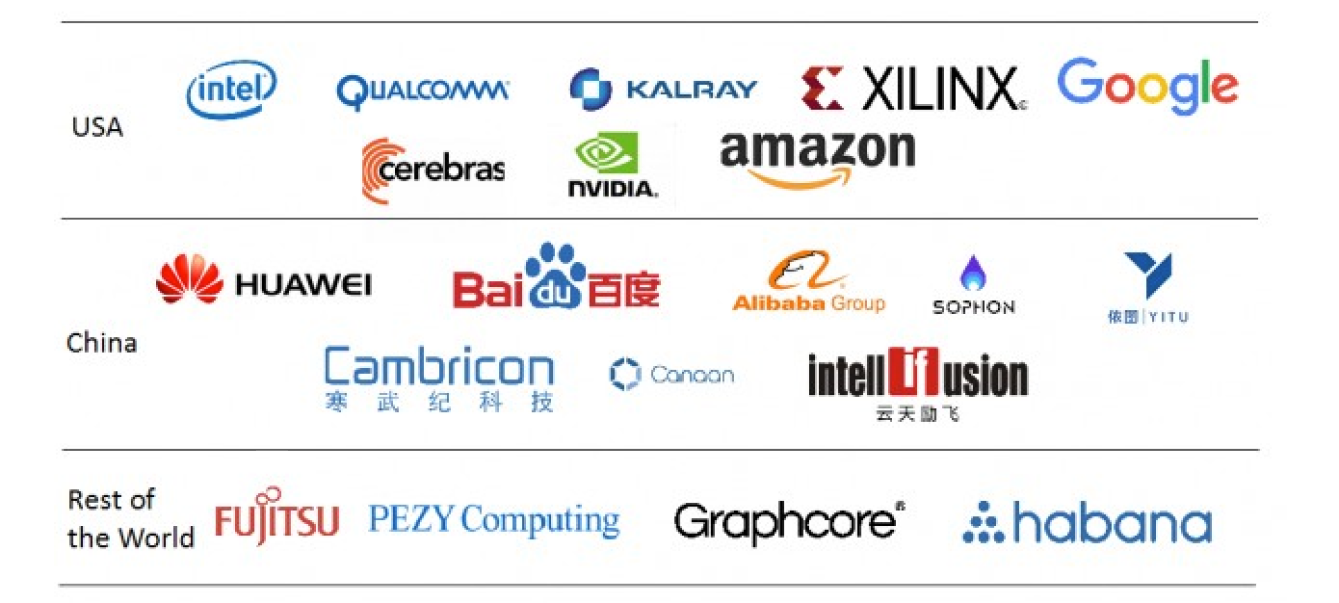
\includegraphics[width=0.5\textwidth]{./figures/Empreses.png}
    \caption{Les capes que te la IA per funcionar}
\end{figure}

\textbf{\Large GPUs}\label{GPUs}\\
Segons \href{https://support.microsoft.com/es-es/windows/todo-sobre-las-unidades-de-procesamiento-gr%C3%A1fico-gpu-e159bedb-80b7-4738-a0c1-76d2a05beab4}{Microsoft} una GPUs és:\\
  La unitat de processament de gràfics (GPU) d'un dispositiu Windows controla el treball relacionat amb els gràfics. Les GPU també es coneixen com a targetes de vídeo o targetes gràfiques.\\
  El treball relacionat amb els gràfics que manegen les GPU inclou els següents elements:
  \begin{itemize}
   \item El grafisme
   \item Efectes
   \item Video
   \item Videojocs
  \end{itemize}
  Hi ha dos tipus bàsics de GPU: GPU integrada i GPU discreta. Coneix els diferents tipus de GPU i troba el que s'ajusta a les teves necessitats:

  \textbf{GPU integrada}
  \begin{itemize}
   \item Les GPU integrades estan integrades directament en el processador principal (CPU).
   \item Les GPU integrades normalment no són tan potents com les GPU discretes, però són més eficients energèticament.
   \item Les GPU integrades sovint són menys costoses que les GPU discretes.
   \item Les GPU integrades permeten que els portàtils siguin més prims, lleugers i eficients.
   \item Les GPU Integrades són excel·lents per a alguns jocs, edició de vídeo lleuger o per treballar amb fotos.
  \end{itemize}

  \textbf{GPU discreta}
  \begin{itemize}
   \item Les GPU discretes són més grans que les GPU integrades i utilitzen més potència, però són les més adequades per a tasques de processament intensiu, com ara edició intensa de fotos i vídeos, treball de disseny i jocs.
   \item En els ordinadors, les GPU discretes són una targeta independent de la CPU, i que es troba en la seva pròpia targeta, fora de la CPU.
   \item Els ordinadors portàtils i tauletes també poden tenir GPU discrets directament a la placa base, però sovint s'afegeixen a la GPU incorporada. La GPU integrada s'utilitza per a tasques gràfiques més lleugeres, mentre que la GPU discreta s'utilitza per a tasques gràfiques més pesades. El canvi entre GPUs a partir de la tasca que es fa permet un equilibri entre rendiment i eficiència energètica.
  \end{itemize}

\subsection{Software i Frameworks}\label{subsec:Software i Frameworks}

\subsubsection{Frameworks}
Segons \href{https://www.inesdi.com/blog/Frameworks-de-IA-que-debes-conocer/}{INESDI}:\\
{\color{gray}``Un Frameworks és, en el camp de la informàtica, una estructura conceptual que proporciona un conjunt d'eines, biblioteques i patrons de disseny per facilitar el desenvolupament de programari. En altres paraules, són marcs de treball que funcionen com un esquelet predefinit, i sobre els quals es pot construir una aplicació o programari.

Pel que fa als seus components, inclouen biblioteques de codi reutilitzables, mòduls predefinits, regles d'arxiu i directori, patrons de disseny i convencions de codificació.''}\\

Un Frameworks, en diferencia, de la biblioteca per el control total que pot tenir el usuari en tema estructura, i organitzacio dels codis, en canvi, una biblioteca està en mans del desenvolupador i només tens accés en els codis que et convenin de la biblioteca. Malgrat la utilitat que propociona no satisfeix la IA de la actualitat i han hagut de desarollar uns Frameworks especifics per la IA, de tal manera en que facilita el desarollament i l'entrenament dels models de la IA.
\subsubsection{Software}
El software és el conjunt de programes, instruccions i regles informàtiques que permeten executar tasques específiques en un ordinador o sistema.

La relació entre el software i la IA funciona de la següent manera: d'una banda, el software dóna utilitat pràctica a la IA en àmbits reals, permetent codificar les seves tècniques i processar les grans quantitats de dades que necessita. D'altra banda, la IA aporta automatització a les tasques repetitives del software, estalviant temps i recursos. Aquesta interacció crea un benefici mutu que forma un cicle perfecte, on cadascú millora i potencia l'altre.

\subsection{Mètodes d'Optimització en Intel·ligència Artificial:Fonaments i Aplicacions}\label{subsec:Optimització i Ajustos}

\subsubsection{Introducció}
La Intel·ligència Artificial (IA) integra múltiples estratègies d'optimització, cadascuna adaptada als diferents models d'IA. A continuació, s'exploren els mètodes més destacades, amb una mini anàlisi dels mecanismes i les referències acadèmiques que hem utilitzat.

\subsubsection{Retropropagació en Aprenentatge Profund}
La retropropagació (\textit{backpropagation}) és com el punt i coma en el text per les xarxes neuronals artificials. Aquest algorisme es basa en un procés iteratiu en dues fases:

\begin{itemize}
\item \textbf{Fase de propagació endavant}: Les dades d'entrada es transmeten a través de les capes de la xarxa, generant una predicció. Durant aquest procés, cada neurona aplica una transformació lineal seguida d'una funció d'activació no lineal, com \textit{\nameref{subsec:1}} o \textit{\nameref{3.7.1}}.

\item \textbf{Fase de propagació enrere}: Es calcula l'error entre la predicció i el valor real utilitzant una funció de pèrdua (\textit{loss function}), com l'error quadràtic mitjà (\textit{Mean Squared Error}) per a problemes de regressió o l'entropia creuada (\textit{Cross-Entropy Loss}) per a classificació. Mitjançant \nameref{subsec:cadena} (\textit{chain rule}), es determina la contribució de cada paràmetre a l'error global, obtenint els gradients $\partial L/\partial W$, on $L$ representa la pèrdua i $W$ els pesos de la xarxa.

\item \textbf{Actualització de paràmetres}: Els pesos s'ajusten en la direcció oposada al gradient, utilitzant variants del descens de gradient, com SGD \textit{\nameref{subsec:gradient}}, que aplica updates amb un subconjunt aleatori de dades, o optimitzadors més sofisticats com Adam (\textit{Adaptive Moment Estimation}), que adapta la taxa d'aprenentatge per a cada paràmetre.
\end{itemize}

Per més informació també podeu accedir aquest  aparatat \ref{subsec:propagació} on també explica la retropropagació de la xarxa neuronal.

\textbf{Suport teòric}:
\begin{quote}
\textit{Rumelhart, D. E., Hinton, G. E., \& Williams, R. J. (1986). ``Learning representations by back-propagating errors.'' Nature, 323(6088), 533-536.}

Aquest article seminal estableix els fonaments matemàtics de la retropropagació, demostrant la seva eficàcia per a l'entrenament de xarxes multicapa.
\end{quote}

\subsubsection{Optimització en Models Generatius}
Els models generatius, com les xarxes generatives adversàries (GANs) i els autoencoders variacionals (VAEs), empren tècniques d'optimització especialitzades:

\paragraph{Xarxes Generatives Adversàries (GANs)}
El marc adversarial de les GANs implica la competició entre dos models:

\begin{itemize}
\item \textbf{Generador (\textit{Generator})}: Transforma un vector de soroll/aleatori(\textit{noise vector}) en dades sintètiques, intentant enganyar el discriminador.

\item \textbf{Discriminador (\textit{Discriminator})}: Distingeix entre dades reals i generades, actuant com un classificador binari.
\end{itemize}

L'entrenament es formula com un joc minimax, on la funció objectiu és:
$ \min_G \max_D V(D, G) = \mathbb{E}_{x \sim p_{\text{data}}}[\log D(x)] + \mathbb{E}_{z \sim p_z}[\log(1 - D(G(z)))] $

La retropropagació s'aplica alternativament amb dues xarxes, ajustant els seus paràmetres per millorar les seves funcions respectives.

\textbf{Suport teòric}:
\begin{quote}
\textit{Goodfellow, I., et al. (2014). ``Generative Adversarial Networks.'' Advances in Neural Information Processing Systems 27 (NeurIPS).}

Aquesta publicació introdueix el concepte de GANs, destacant el seu potencial per a la generació de dades realistes mitjançant aprenentatge adversarial.
\end{quote}

\paragraph{Autoencoders Variacionals (VAEs)}
Els VAEs optimitzen l'\textit{Evidence Lower Bound} (ELBO), que combina dos termes:

\begin{itemize}
\item \textbf{Terme de reconstrucció}: Minimitza l'error entre les dades originals i les reconstruïdes.

\item \textbf{Terme de regularització}: Minimitza la divergència de Kullback-Leibler (\textit{KL divergence}) entre la distribució latent i una distribució prior (normalment una normal estàndard).
\end{itemize}

L'optimització es realitza mitjançant gradient descent sobre l'ELBO, amb l'ajut del \textit{reparameterization trick} per a un càlcul eficient dels gradients.

\textbf{Suport teòric}:
\begin{quote}
\textit{Kingma, D. P., \& Welling, M. (2013). ``Auto-Encoding Variational Bayes.'' arXiv preprint arXiv:1312.6114.}

Els autors presenten el marc teòric dels VAEs, introduint tècniques clau com el \textit{reparameterization trick} per a l'entrenament eficient de models generatius probabilístics.
\end{quote}

\subsubsection{Aprenentatge per Reforç i Optimització basada en Polítiques}
En l'aprenentatge per reforç (\textit{Reinforcement Learning, RL}), l'optimització es centra en maximizar la recompensa acumulada. Un enfocament prominent és el \textit{Policy Gradient}, que ajusta directament la política (\textit{policy}) mitjançant:
\[ \nabla_\theta J(\theta) = \mathbb{E}_{\tau \sim \pi_\theta} \left[ \sum_{t=0}^T \nabla_\theta \log \pi_\theta(a_t|s_t) \cdot R(\tau) \right] \]
on $\tau$ representa una trajectòria i $R(\tau)$ la recompensa acumulada.

\textbf{Suport teòric}:
\begin{quote}
\textit{Sutton, R. S., et al. (2000). ``Policy Gradient Methods for Reinforcement Learning with Function Approximation.'' Advances in Neural Information Processing Systems 12 (NeurIPS).}

Aquest treball estableix les bases teòriques dels mètodes de gradient de polítiques, demostrant la seva aplicabilitat en entorns complexos.
\end{quote}

\subsubsection{Alternatives a la Retropropagació: Algorismes Evolutius}
Per a problemes on el càlcul de gradients no és factible, els algorismes genètics (\textit{Genetic Algorithms, GA}) ofereixen una solució viable. Aquests algorismes emulen l'evolució natural mitjançant:

\begin{itemize}
\item \textbf{Selecció}: Els individus més aptes (\textit{fitness}) tenen major probabilitat de reproduir-se.

\item \textbf{Creuament (\textit{Crossover})}: Combina característiques de dos individus per generar descendència.

\item \textbf{Mutació}: Introdueix variabilitat genètica aleatòria.
\end{itemize}

\textbf{Suport teòric}:
\begin{quote}
\textit{Holland, J. H. (1975). ``Adaptation in Natural and Artificial Systems.'' University of Michigan Press.}

Holland formalitza els algorismes genètics, inspirant-se en els mecanismes de selecció natural per a resoldre problemes d'optimització complexos.
\end{quote}

\subsection{Ètica i Regulació}\label{subsec:Ètica i Regulació}

Un cop enteses totes les funcionalitats i capacitats de la intel·ligència artificial (IA), és fonamental aplicar-hi principis d’ètica i moral. Encara que la IA no sigui un ésser viu, és una eina creada per els  humans, i per tant cal establir-hi limitacions per evitar-ne els mals usos i garantir el respecte als drets humans i a la privacitat. Aquesta part és crucial en el desenvolupament d’una IA responsable. En aquest sentit, molts estats i organismes ja han publicat diverses lleis legítimes i regulacions. Algunes de les més rellevants són:
 \begin{itemize}
  \item \textbf{Llei d’IA de la Unió Europea (AI Act):} És la primera regulació integral sobre la IA. Classifica els sistemes d’IA segons el seu nivell de risc (inacceptable, alt, limitat i mínim) i estableix requisits estrictes per als usos d’alt risc, com la transparència, supervisió humana i seguretat.
  \item \textbf{Reglament General de Protecció de Dades (GDPR):} Tot i no ser exclusiu per a la IA, aquest reglament europeu protegeix la privacitat i les dades personals dels ciutadans. És clau en el desenvolupament d’IA que utilitza dades personals.
  \item \textbf{Principis ètics de la UNESCO sobre la IA (2021): Proposen una base global per al desenvolupament ètic de la IA, centrant-se en el respecte pels drets humans, la igualtat, la sostenibilitat, la no discriminació i la supervisió humana.}
  \item \textbf{Guies de l’OCDE sobre la IA:}Recomanen que els sistemes d’IA siguin transparents, responsables, segurs i que promoguin el benestar de la societat, ajudant a establir marcs internacionals de bones pràctiques.
 \end{itemize}



Fonts:\href{https://blogs.uoc.edu/digitapia/the-european-unions-artificial-intelligence-act-explained/}{Bloc IA} \href{https://formaciooberta.eapc.gencat.cat/contingutsdelscursos/tdp/080_int_artificial/inici.html}{EAPC Wiki}
\href{https://www.ibm.com/think/topics/machine-learning}{IBM ML} \href{https://www.ultralytics.com/es/blog/understanding-the-impact-of-compute-power-on-ai-innovations}{La relació que estableix entre la IA i el maquinari }\cite{bengio2012} \href{https://digital-strategy.ec.europa.eu/en/policies/regulatory-framework-ai?utm_source=chatgpt.com}{AI ACT} \href{https://www.unesco.org/en/legal-affairs/recommendation-ethics-artificial-intelligence?utm_source=chatgpt.com}{IA UNESCO}

\section{Que és una xarxa neuronal artificial/biologica?}\label{sec:xarxa neuronal}
Una xarxa neuronal artificial és un model computacional inspirat en el funcionament del cervell humà, utilitzat en el camp de la intel·ligència artificial (IA) i l'aprenentatge automàtic (machine learning). Està dissenyada per reconèixer patrons, prendre decisions i aprendre a partir de dades, sense ser programada explícitament per a cada tasca específica.
Si tenim una artificial també tindrem una biològica. Una xarxa neuronal biològica es refereix al sistema interconnectat de neurones (cèl·lules nervioses) en el cervell i el sistema nerviós dels éssers vius. Aquestes xarxes són la base de la cognició, l'aprenentatge i les funcions biològiques en humans i animals.
Aquí hi és una taula de comparació entre una biologica i artificial:

\begin{table}[h!]
\begin{tabular}{|l|l|l|}
\hline
\textbf{Aspecte} & \textbf{Xarxa neuronal biològica} & \textbf{Xarxa neuronal artificial} \\ \hline
\textbf{Base} & Cèl·lules vives (neurones). & Algoritmes matemàtics. \\ \hline
\textbf{Energia} & Baix consum (\textasciitilde20 watts). & Alt consum (GPUs/TPUs). \\ \hline
\textbf{Aprenentatge} & Plasticitat sinàptica. & Backpropagation + dades. \\ \hline
\textbf{Velocitat} & Lent (mil·lisegons). & Ràpid (nanosegons). \\ \hline
\end{tabular}
\caption{Comparativa entre xarxes neuronals biològiques i artificials}
\end{table}
Fons: \href{https://www.ibm.com/docs/es/spss-modeler/saas?topic=networks-basics-neural}{https://www.ibm.com/docs/es/spss-modeler/saas?topic=networks-basics-neural}
\section{Estructura d'una xarxa neuronal}\label{sec:3.6}
Una xarxa neurnal combina diverses capes de procesament i utilitza elements simples que operen en paral·lel, simulen i estan inspirades en els sistemes nerviosos biològics com hem explican en l'apartat \ref{sec:xarxa neuronal}. Consta d'una capa d'entrada, seguit d'una o varies capes ocultes i finalment una capa de sortida. Les capes estan interconectades mitjançant nodes o neurones; cada capa utilitza la sortida de la capa anterior com a entrada.

\begin{itemize}
 \item \textbf{Capa d'entrada:}La capa d'entrada és la primera capa que reb directament la informació d'entrada que es prcessarà. Aquesta capa no realitzarà càlculs complexos, simplement transmet les dades a les capes seguents per fer el processament.
 \item \textbf{Capes ocultes:}Les capes ocultes són les capes que estan entre la capa d'entrada i la de sortida, aquestes capes contenen unitats no observables. La seva funció principal és processar les dades de la capa d'entrada per extraure característiques i patrons complexos. Aquestes capes són els que realitzan els càlculs i permet que la xarxa aprengui relacions no lineals i representacions abstracts de les dades, això és molt important per fer tasques complexes com el reconeixement de patrons. La quantitat de neurones que hi ha en les capes ocultes és un factor determinant per la capacitat que tingui la xarxa per capturar dades complexes.
 \item \textbf{Capa de sortida:}La capa de sortida és l'última capa que forma una xarxa neuronal i és l'encarregada de produïr la predicció final del model. Aquesta capa utilitza la informació que ha processat la o les capes ocultes i la transforma a travès d'una funció activa per generar una sortida, que pot ser una predicció numèrica, una clasificació o qualsevol altre resultat. Les neurones d'aquesta capa estan connectades amb totes les neurones de la capa anterior.
 \end{itemize}


\begin{figure}[h!]
    \centering
    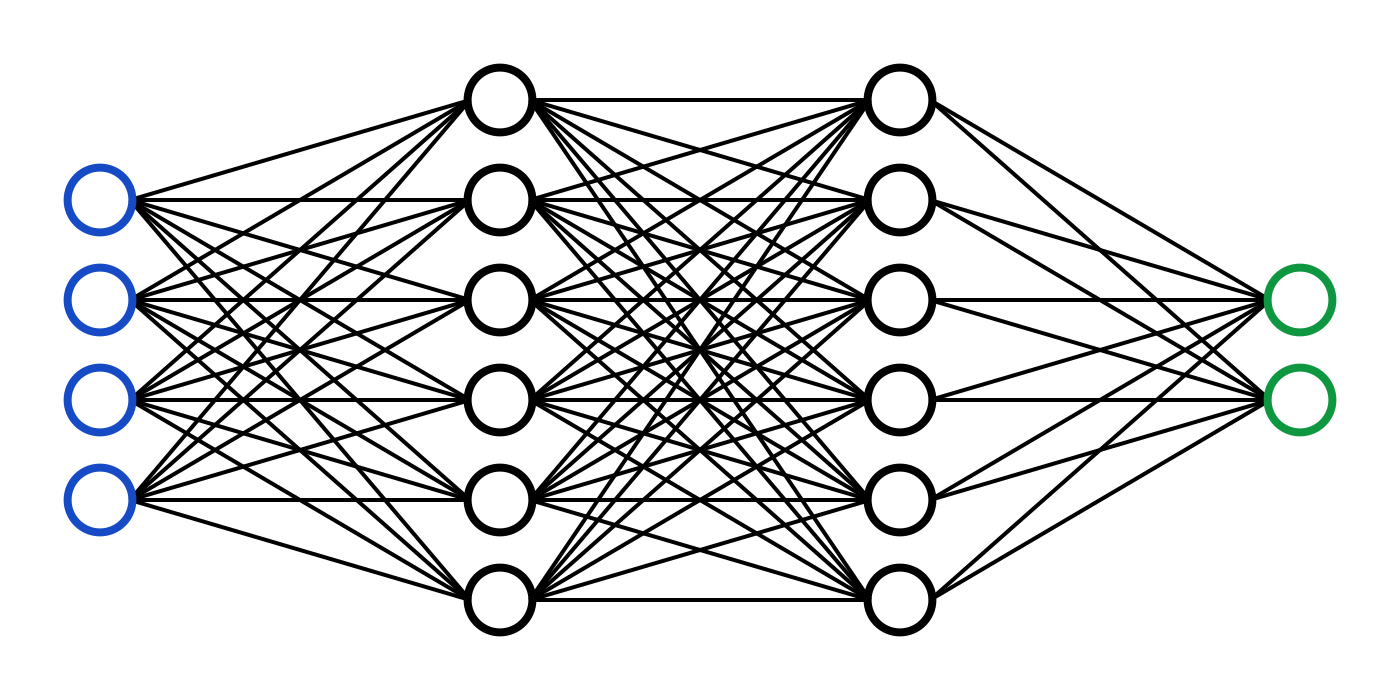
\includegraphics[width=0.5\textwidth]{./figures/xarxa.png}
    \caption{Estructura d'una xarxa neuronal}
\end{figure}

Fons: \href{https://msmk.university/hidden-layer/}{https://msmk.university/hidden-layer/}

\href{https://www.linkedin.com/advice/0/what-some-examples-linear-nonlinear-models-real-world?lang=es&lang=es&originalSubdomain=es}{Article Linkedin}

\section{
Funció d'activació}\label{sec:3.5.3}
Les funcions d'activació són un component integral de les xarxes neuronals que els permeten aprendre patrons complexos en les dades. Transformen el senyal d'entrada d'una neurona en un senyal de sortida que passa a la capa següent. Sense funcions d'activació, les xarxes neuronals es limitarien a modelar únicament relacions lineals entre entrades i sortides, és a dir, introdueixen la no linealitat i produeixen la sortida de la neurona.

\subsection{Funció sigmoide}\label{3.7.1}
Una funció d'activació molt coneguda és la funció sigmoide. La seva fórmula és:
\[ \sigma(x) = \frac{1}{1 + e^{-x}} \]

Aquesta funció matemàtica transforma qualsevol valor d'entrada real en un valor que està 0 i 1. La seva forma característica és una curva en forma de ``S''. Si el valor de $x$ que introduïm a la funció és molt gran o fins infinit $(\infty)$, llavors\ $\sigma$ serà 1; en canvi si és molt petit o menys infinit $(-\infty)$,\ $\sigma$ serà 0, i si x = 0,  $\sigma$  serà 0,5.

\begin{figure}[h!]
    \centering
    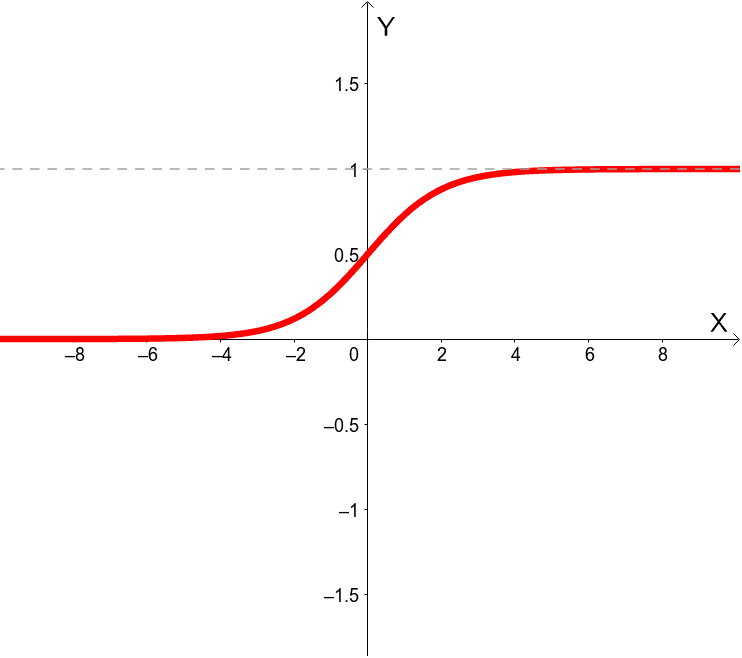
\includegraphics[width=0.5\textwidth]{./figures/grafica_sigmoide.png}
    \caption{Gràfica de la funció sigmoide}
\end{figure}

\textbf{Avantatges:}
La avantatge principal de la funció sigmoide és la seva suavitat i la facilitat de derivació. La funció és diferenciable en tots els punts, cosa que facilita el càlcul de gradients, això vol dir que permet als algoritmes d'optimització treballar amb la funció de manera eficient. A més, la funció és monòtona creixent, ho que significa que una entrada major sempre produirà una sortida major, fent que sigui útil per modelar relacions de causa i efecte.

\textbf{Desavantatges:}
Tanmateix, la funció sigmoide també té algunes desavantatges. Un dels seus problemes és que la funció es satura els gradients. Quan els valors d'entrades són grans, ho que significa que la derivada de la funció s'apropa a 0 i l'aprenentatge es relentitza. Un altre problema és que aquesta funció no és simètrica, causant a les entrades negatives i positives es processin de mandera diferent, això pot afectaral rendiment de la xarxa. Tot això dificulta el procès d'entrenament de la xarxa en la ràpida minimització de la funció d'error utilitzant l'algoritme de Gradient Descendent.
\subsection{Funció ReLU(Funció Uniat Rectificada Uniforme)}\label{subsec:1}
La funció Unitat Rectificada Uniforme té la fòrmula seguent:
\[ f(x) = \max(0, x) \]

Aquesta funció té l'algoritme seguent: Si el valor d'entrada es menor que 0, mostra 0, si el valor d'entrada es major o igual que 0, mostrarà el valor d'entrada. Això vol dir que la funció és lineal si la entrada és més gran que 0 perquè la pendent és 1. Encara que la funció ReLU és lineal per a la mitat del seu espai d'entrada, tècnicament és una funció no lineal perquè té un punt no diferenciable en x = 0, on canvia bruscament respecte a x. Aquesta no linealitat permet a les xarxes neuronals apendre patrons complexos.

\begin{figure}[h!]
    \centering
    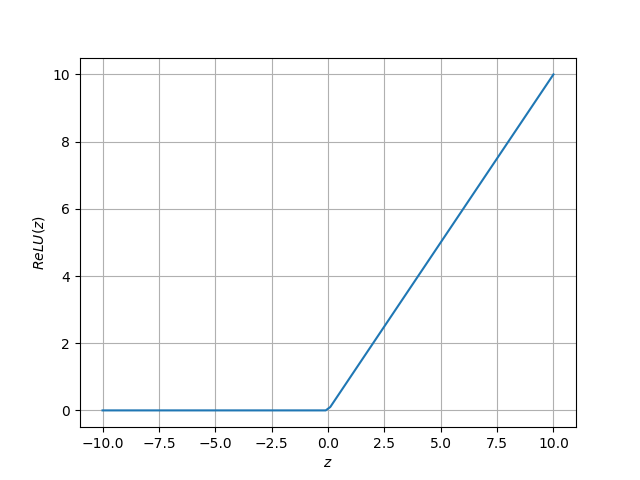
\includegraphics[width=0.5\textwidth]{./figures/ReLU.png}
    \caption{Gràfica de la funció ReLU}
\end{figure}

Tot i això, aquesta funció té una desavanantatge; si utilitzen la funció ReLU com a funció d'activació pasarà una cosa, i es que tots els valors negatius són 0, per tant en el procès de retropropagació, explicat a l'apartat \ref{subsec:retropropagació}, no es produeix els valors d'ajust en les neurones negatives. Per solucionar aquest problema s'ha inventat una nova funció que es diu Leaky ReLU. Funciona igual com l funció ReLU, però té un valor determinat per les neurones negatives.

\begin{figure}[h!]
    \centering
    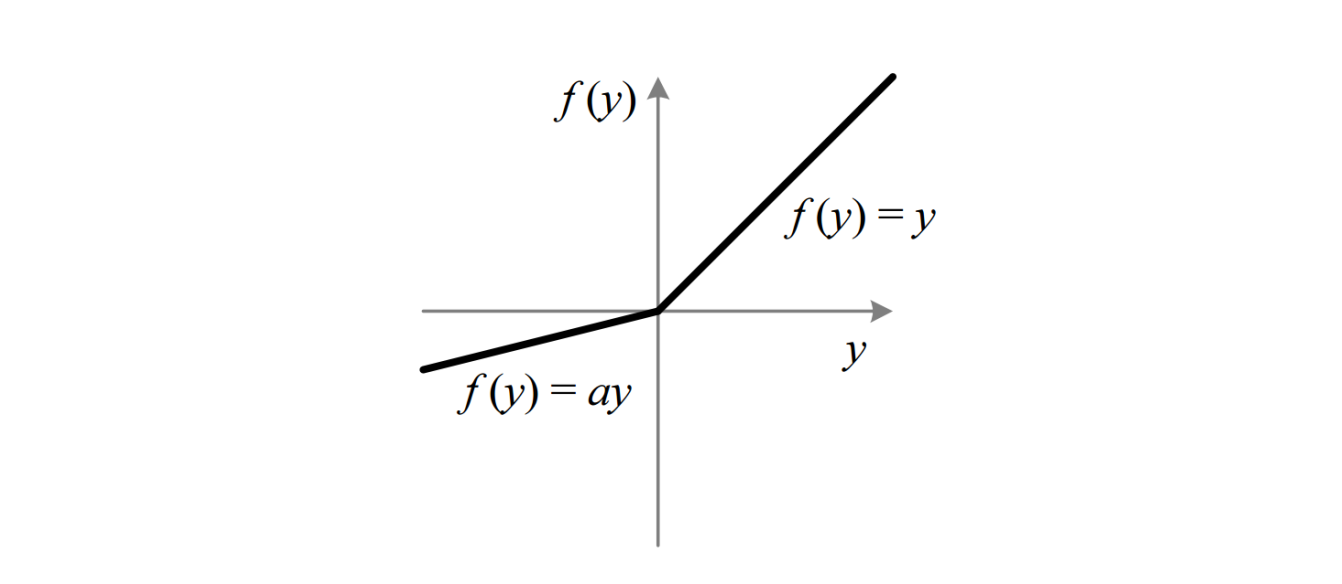
\includegraphics[width=0.5\textwidth]{./figures/leaky_ReLU.png}
    \caption{Gràfica de la funció Leaky ReLU}
\end{figure}

\subsection{Funció Softmax}
La funció Softmax, és una de les funcions que més s'utilitzen en xarxes neuronals i és especialment útil en el context dels problemes de clasificació multiclase. Aquesta funció opera sobre un vector que representa les previsions de cada clase, calculades per les capes anterior.

\begin{figure}[h!]
    \centering
    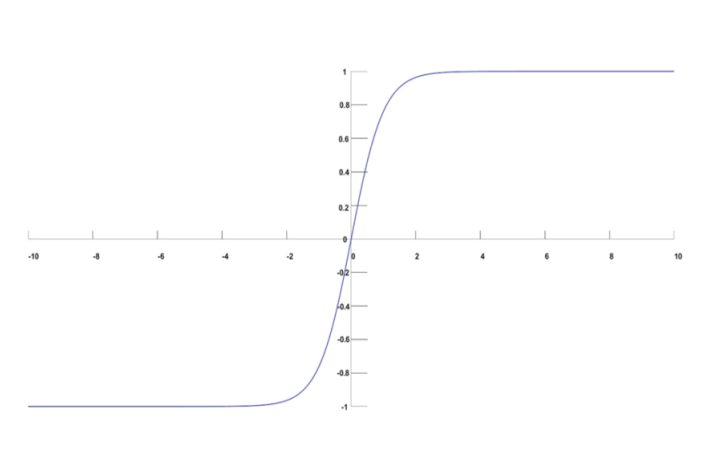
\includegraphics[width=0.5\textwidth]{./figures/Softmax.png}
    \caption{Gràfica de la funció Softmax}
\end{figure}

Per a un vector d'entrada x amb elements x1, x2,..., xC, la funció Softmax es defineix com:
\[f(x_i) = \frac{e^{x_i}}{\sum_{j=1}^{n} e^{x_j}}\]

El resultat de la funció Softmax és una distribució de probabilitat de la quàl la suma és 1. Cada element del resultat representa la probailitat de que l'entrada pertanyi a una clase determinada. L'ús d'aquesta funció garantitza de que tots els valors de la sortida siguin positius. Això és molt important perquè les porbabilitats no poden ser negatives.

\begin{figure}[H]
    \centering
    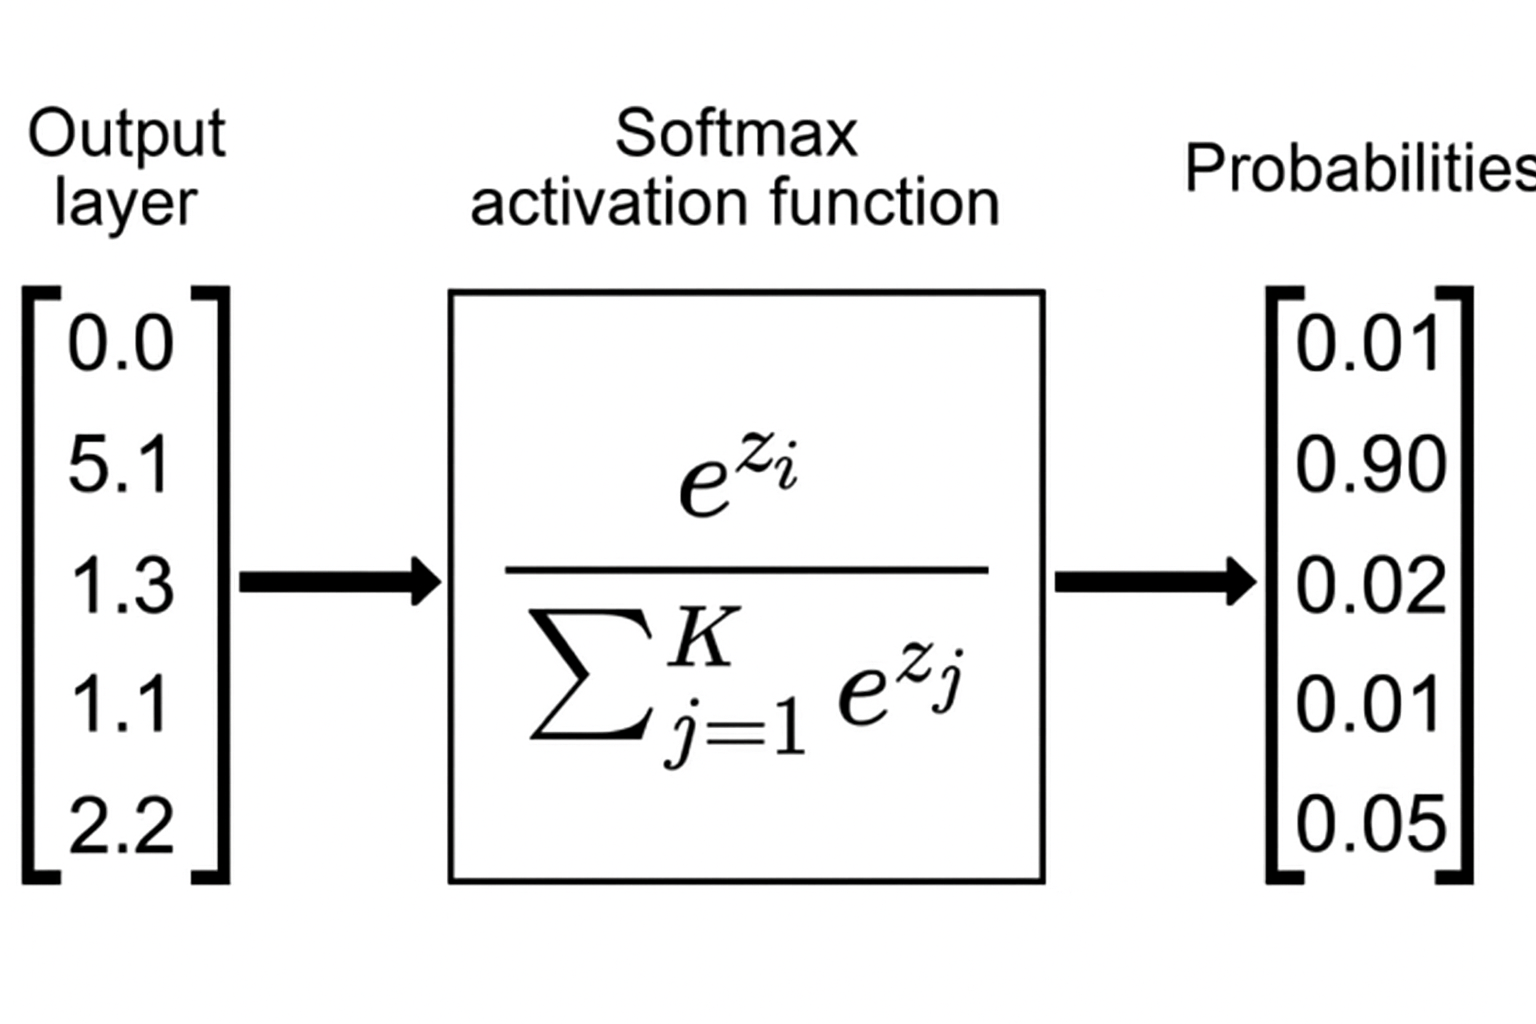
\includegraphics[width=0.5\textwidth]{./figures/representacio_Softmax.png}
    \caption{Representació de la funció Softmax}
\end{figure}

Fons: \href{https://msmk.university/hidden-layer/}{https://msmk.university/hidden-layer/}


\href{https://jacar.es/la-funcion-sigmoide-una-herramienta-clave-en-redes-neuronales/}{https://jacar.es/la-funcion-sigmoide-una-herramienta-clave-en-redes-neuronales/}

\section{Com funciona una xarxa neuronal?}\label{sec:3.8}
Ara que sabem quina estructura forma una xarxa neuronal artificial, toca entendre com funciona. Les neurones o nodes son els pilars més importants d'una xarxa neuronal. Cada neurona utilitza la entrada, la processa fent una suma ponderada entre els pesos i les entrades, després una funció d'activació, i pasa la sortida a altres neurones.

Les conexions(pesos i biaixos) son la força de conexió entre dos neurones representades per un pes.
Els pesos: Son valors que determinen cuánta influència té la producció d'una neurona sobre un altre, marca la importància que té cada neurona.
Els biaixos: Són paràmetres adicionals que ajuda a ajustar els valors de les neurones. És un valor capaç d'apendre com el pes, això vol dir que el model pot utilitzar l'algoritme de retropropagació per a millorar els valors com per exemple els pesos i biaixos.
El umbral: Si la sortida de qualsevol node individual és més gran que el valor del umbral, aquell node s'acivarà i envia dades a la seguent capa de la xarxa. En cas contrari, no es pasa ninguna dada a la seguent capa de la xarxa.

Hem de pensar en que cada node individual com el seu propi model de regressió lineal, compost per dades d'entrada, ponderacions, un umbral o un biaix, i una sortida. La fórmula per calcular els valors d'una xarxa neuronal és la seguent:

\[
\sum w_i x_i + \text{biaix} = w_1 x_1 + w_2 x_2 + w_3 x_3 + \text{biaix}
\] \\

$w_i$: Pesos\\
$x_i$: Entrades\\


Per entendre-ho millor, donarem un exemple: Imagina que vols anar a la platja a fer surf i la teva decisió dependrà d'aquestes 3 preguntes:\\

Hi ha oles?\\
Hi ha poca gent?\\
Hi ha tauros?\\

Analitzarem en detall com funciona un sol node de la xarxa neronal, utilitzant únicament valors binaris (0 y 1) com entrades, 0 voldrà dir ``No'' y 1 ``sí''.
LLavors suposent el següent cas:

$x_1$ = 1, les oles són bones\\
$x_2$ = 0, hi ha molta gent a la platja\\
$x_3$ = 1, Sí que tinc temps\\

Ara, hem d'asignar algunes ponderacions per determinar la importància. Unes ponderacions majors significan que determinades variabbles son més importants per la decisió.

$w_1$ = 5, hi ha d'haveri moltes oles per poder surfejar\\
$w_2$ = 2, no t'importa que hi hagi molta gent\\
$w_3$ = 4, tens pors als taurons \\

Per últim, ambé suposem un valor umbral de 3, ho que es traduiria en un valor de biaix de -3. Amb totes aquestes entrades, ja podem substituir els valors en la nostre fòrmula per obtenir la sortida.

Fonts: \href{https://www.ibm.com/es-es/think/topics/neural-networks}{IBM} i \href{https://aws.amazon.com/es/what-is/neural-network/}{Amazon Web Services}

Les xarxes neuronals operen a travès d'un procès de dos pasos: La propagació directa i la retropropagació.

\subsection{Propagació cap a davant}\label{subsec:propagació}
Durant la propagació cap a davan, les dades ingresen en la xarxa a travès de la capa d'entrada i flueixen secuencialment a travès de les capes ocultes fins a la capa de sortida. En cada neurona, els valors d'entrada del model es multiplican per els seus pesos corresponents i es sumen. Aquesta suma ponderada es pasa a travès d'una funció d'activació, explicada prèviament a l'apartat \ref{sec:3.5.3}. Aquest procès continua capa per capa, això acaba conduïnt cap a la predicció final en la capa de sortida.

Aquest procès és important per les seguents raons:
\begin{itemize}
 \item \textbf{Base per l'aprenentatge:} No es pot comprendre com aprenen les xarxes neuronals sense primer entendre com fan prediccions. La programació cap a davan és el requisit prèvi que s'ha de coneixer per comprendre la \nameref{subsec:retroprgramació}, l'algoritme que permet l'aprenentatge.
 \item \textbf{Optimització:} En el cas de que una xarxa neuronal no funcioni bé, saber com flueixen les dades per la xarxa t'ajudarà a identificar i solucionar problemes.
 \item \textbf{Diseny del model:} Un diseny eficaç de la xarxa requereix comprendre com es distribueix la informació a travès de les configuracions de capes.
\end{itemize}

\section{Retropropagació en les xarxes neuronals}\label{subsec:retropropagació}
Mentre que la programació directa fa prediccions, la retroporgramació és la forma en que la xarxa apren d'errors. Implica comparar la predicció de la xarxa amb el valor objectiu real i calcular un terme d'eror mitjançant una funció d'error.
Aquest error es propaga enrere a travès de la xarxa, començant des de la capa de sortida. Durant aquest procès, la xarxa ajusta els pesos i els biaixos de cada connexió en funció de la seva contribució a l'error, amb l'objectiu de minimitzar-lo.
Aquest procès iteratiu de càlcul d'erros i ajustament de pes permet a la xarxa d'aprenentatge profund millorar gradualment les seves prediccions.
El procès de retropropagació es basa en el principi d'optimització del gradient descendent, explicat anteriorment en l'apartat \ref{subsec:gradient}, es calculen els gradients d'error respecte als paràmetres de la xarxa en sentit contrari i en cada capa. Per aquesta tasca, s'utilitza l'algoritme de la cadena (\ref{subsec:cadena}) per propagar l'error cap enderrere desde la sortida fins l'entrada.

\subsection{Com funcona la retropropagació?}
El funcinament de la retropropagació el podem dividir en 5 fases. Cada un d'es possibilita a la xarxa neuronal apendre de manera eficient a partir de dades proporcionats. Les fases són les seguents:
\begin{itemize}
 \item \textbf{Propagació cap endevant:} Aquesta fase inicial és on s'introdueixen les dades de prova en la xarxa neuronal desde la capa d'entrada fins a la sortida.
 \item \textbf{Càlcul d'error:} Una vegada s'obté la sortida de la xarxa, es compara amb el valor desitjat mitjantçant una funció d'error. Aquesta funció quantifica la discrepança que s'ha produït entre la predicció i el valor real.
 \item \textbf{Retropropagació de l'error:} En aquesta fase els gradients de l'error es calculan respecte a cada paràmetre en la xarxa. Com em dit abans, aquest procès comença de manera inversa a la propagació, desde la sortida fins l'entrada.
 \item \textbf{Actualització dels paràmetres:} Una vegada que s'ha calculat els gradients de l'error en tots els paràmetres, aquestos s'actualitzan. D'aquesta manera, els errors en la predicció es minimitzan de manera gradual en cada iteració de l'entrenament.
 \item \textbf{Configuració de la predicció:} Després de totes les optimitzacions, el mètode de càlcul torna a revisar les entrades de proba. Després de tot això, es busca garantizar els resultats esperats.
\end{itemize}
\subsection{Avantatges de la retropropagació}
La retropropagació ofereix unes avantatges que l'han convertit en una eina fonamental en l'entrenament de les xarxes neuronals. Les seves avantatges són les seguents:

\begin{itemize}
 \item \textbf{Eficiència en l'optimització de parámetres:} Gracies al càlcul de gradient mitjantçant la regla de la cadena, explicada a l'apartat \ref{subsec:cadena}, la retropropagació facilita l'ajust dels paràmetres d'una xarxa neuronal de manera eficient. Això s'aconsegueix determinant la contribució de cada variable al error total de la xarxa, ho que augmenta notablement a l'hora de fer prediccions precises.
 \item \textbf{Flexibilitat en l'arquitectura:} La retropropagació és compatible en moltes varietats d'arquitectura en les xarxes neuronals, com l'aprenentatge profund amb múltiples capes ocultes. Aquesta característica permet disenys que s'adapten millor a la complexitat de dades i les necesitats de cada tasca.
 \item \textbf{Escalabilitat:} Es posible augmentar la retropropagació perquè traballi amb moltes dades i xarxes neuronas molt grans, ja que hi haurà vegades en que una xarxa pot tindre fins a milions de paràmetres, això exigeix una gestió eficient.
 \item \textbf{Optimització continua:} La retropropagació ofereix la actualització contínua de les variables durant l'entrenament. És un ajust dinàmic important per millorar poc a poc el rendiment de la xarxa amb cada iteració i nous cicles d'aprenentatges.
\end{itemize}
Fonts: \href{https://www.universidadviu.com/es/actualidad/nuestros-expertos/como-funciona-un-algoritmo-de-backpropagation#que-es-backpropagation}{Universitat internacional de valència} i \href{https://msmk.university/backpropagation/}{Universitat de ciències i tecnologia}


\subsection{La regla de la cadena}\label{subsec:cadena}

En l'aprenentatge automàtic, sovint es treballa amb funcions compostes complexes que depenen de diversos paràmetres i capes. Per tal de facilitar el càlcul dels gradients i optimitzar el rendiment computacional, s'utilitza la \textbf{regla de la cadena}.

La regla de la cadena és una tècnica de derivació matemàtica que permet descompondre la derivada d'una funció composta en el producte de derivades de les seves funcions internes. D’aquesta manera, es poden calcular les derivades de manera escalonada i eficient, especialment en el context de l’algorisme de propagació enrere (backpropagation).

Per exemple, si tenim una funció composta de la forma:

\[
L = f(g(h(x)))
\]

La derivada de \( L \) respecte a \( x \) s'obté aplicant la regla de la cadena:

\[
\frac{dL}{dx} = \frac{df}{dg} \cdot \frac{dg}{dh} \cdot \frac{dh}{dx}
\]

Aquest procediment és fonamental per entrenar xarxes neuronals, ja que permet calcular com cada pes de la xarxa contribueix a l'error global, i així ajustar-los mitjançant tècniques com el descens de gradient.

fonts:\href{https://medium.com/%40ppuneeth73/the-chain-rule-of-calculus-the-backbone-of-deep-learning-backpropagation-9d35affc05e7}{Medium deep machine-learning} \ \href{https://www.geeksforgeeks.org/machine-learning/chain-rule-derivative-in-machine-learning/}{Greek machine-learning}



